\chapter{Walidacja rozwiązania}
\label{cha:tests}
Po wstępnym nastrojeniu układu, należy uruchomić oraz przetestować urządzenie. Autor zapoznał się w~tym celu z~normą dotyczącą mierzenia poziomu natężenia hałasu \cite{test_norm}, jednak ze względów subiektywnych nie zastosował się do niej, a~obrał własną metodę wykonania testu. Ze względu na niskie amplitudy sygnałów występujących w~urządzeniu i~podczas testu, autor zdecydował się przetestować urządzenie rejestrując sygnały przy użyciu oscyloskopu cyfrowego z~pamięcią. Zarówno sposób, jak i~wyniki pomiarów, opisane są w~sekcji \ref{sec:practical_test}.
\section{Typowe rodzaje hałasu}
Jak już wspomniano w~sekcji \ref{sec:hałas} rozdziału \ref{cha:teoria}, typowymi rodzajami hałasu, które można chcieć tłumić takim urządzeniem, są:
\begin{itemize}
	\item rozmowy pobliskich osób,
	\item szum wentylacyjny,
	\item dźwięk towarzyszący pracy silnika.
\end{itemize}
Są to zatem sygnały charakteryzujące się (w~przybliżeniu) stałym przedziałem częstotliwościowym i~niewielkim natężeniem, jednak będące uciążliwymi w~dłuższej perspektywie czasowej. W~ramach testu praktycznego sprawdzono działanie układu przy ekspozycji na dźwięk pochodzący od sygnałów sinusoidalnych, złożeń kilku takich sygnałów (np. sygnał sinusoidalny o~częstotliwości \SI{200}{\Hz} + \SI{700}{\Hz}), sygnałów prostokątnych oraz użyto sygnału z~wobulatora (przemiatanie częstotliwości), aby sprawdzić wpływ przegrody dźwiękochłonnej na pracę układu. Testowane sygnały często stanowią część składową hałasów wymienionych wcześniej.
\section{Test praktyczny}
\label{sec:practical_test}
\subsection{Warunki testu}
\label{subsec:circumstances}
Układ został przetestowany w~pomieszczeniu przeznaczonym dla prowadzenia zajęć laboratoryjnych. W~trakcie przeprowadzania testu nie występowały inne, znaczące źródła hałasu, które mogłyby w~niekontrolowany sposób zakłócać pracę układu i~pomiar. Do akwizycji sygnałów obecnych bezpośrednio na~połączeniach układu zastosowano oscyloskop cyfrowy, w~którym wykorzystano 3~kanały pomiarowe. Kanał pierwszy (żółty) podłączono do sygnału mikrofonu głównego, aby zmierzyć poziom hałasu bez tłumienia. Kanał drugi (niebieski) oscyloskopu podłączony został do sygnału pochodzącego z~mikrofonu odsłuchowego, zaś ostatni z~kanałów (różowy) użyty został do zmierzenia napięć obecnych na połączeniu wyjścia przetwornika C/A ze wzmacniaczem głośnikowym. Pozwoliło to na bezpośredni i~jednoczesny podgląd trzech kluczowych zmiennych. W~zależności od potrzeby, włączano lub wyłączano algorytm i~w~obu przypadkach zapisywano dane pochodzące z~urządzenia pomiarowego celem opracowania ich na komputerze~PC.

Głośnik użyty do odgrywania dźwięków imitujących hałas zewnętrzny podłączono do generatora funkcyjnego i~umieszczono go w~bliskiej odległości od mikrofonu głównego zbudowanego urządzenia. Odległość od źródła dźwięku wynosiła \SI{45}{\mm}, zaś czas pomiaru był zmienny dla każdego z~etapów, co wynika bezpośrednio z~ilości czasu, jaką zajmuje strojenie filtra dla bardziej złożonych sygnałów. Ostatecznie, w~ramach każdego etapu testu, czekano aż filtr nastroi się względem podawanego hałasu, by następnie zapisać dane z~oscyloskopu cyfrowego.

Należy przypomnieć, że celem zamodelowania nieidealnego przylegania słuchawek do głowy użytkownika, zastosowano element dystansowy w~postaci długopisu, rozdzielający muszle nauszników. Powoduje to lekkie zwiększenie poziomu natężenia hałasu, jaki dociera do mikrofonu odsłuchowego oraz uwydatnia działanie aktywnej części projektu autora. 
\subsection{Wyniki testu}
Celem sprawdzenia jakości zbudowanego urządzenia, dokonano testu praktycznego, gdzie w~pomieszczeniu laboratoryjnym zmierzono poziom natężenia hałasu słyszanego przez mikrofony urządzenia. Do generowania dźwięków testowych użyto głośnika podłączonego do generatora funkcyjnego. Łącznie dokonano siedmiu pomiarów z~akwizycją sygnału w~dwóch wariantach -- tylko z~tłumieniem pasywnym lub jednoczesnym pasywnym i~aktywnym pochodzącym z~zaprogramowanego układu. Podczas testów tłumienia aktywnego, po pewnym czasie działania i~uczenia algorytmu, odczytywano wagi filtra LMS, co pozwoliło wyznaczyć jego odpowiedź impulsową.

Podczas przeprowadzania testu, doświadczalnie wyznaczono, że efektywnym zakresem aktywnego tłumienia hałasu jest pasmo częstotliwościowe od około \SI{400}{\Hz} do około \SI{820}{\Hz}. Okazuje się, że poniżej dolnej granicy pasma, do głosu zaczynają dochodzić nieliniowości zawieszenia membrany głośnika oraz częstotliwości rezonansowe użytych komponentów. Można częściowo zmniejszyć wpływ tych czynników na pomiar poprzez zmniejszenie amplitudy podawanego hałasu, wtedy jednak szumy wewnątrz-układowe zaczynają stanowić znaczącą część sygnału. Niewykluczone również, że kształt i~rozmiar przestrzeni wewnątrz muszli użytej słuchawki może powodować powstawanie fal stojących, gdzie dla pewnych częstotliwości mikrofon odsłuchowy mógłby się znaleźć w~strzałce lub węźle --  a~to mocno wpływałoby na odczytywane wartości i~powodowałoby rozstrojenie filtra. Z~kolei powyżej górnej granicy pasma aktywne tłumienie traciło swą efektywność na rzecz tłumienia pasywnego. Choć można było próbować dokonywać pomiarów dla wyższych częstotliwości hałasu, to autor w~chwili testu nie dysponował przyrządami pomiarowymi o~wyższej dokładności i~mniejszym zaszumieniu. Z~tych powodów uznano, że wymieniony zakres będzie odpowiednio dobrym punktem startowym urządzenia, gdzie można już zauważyć efekty działania projektu, jednak wciąż pozostaje dużo możliwości jego poprawy.

W~związku z~takimi możliwościami prototypu, dokonano następujących siedmiu pomiarów, w~których parametry sygnału z~generatora funkcyjnego zasilającego głośnik imitujący zewnętrzne źródło hałasu zapisano na początku w~informacji testu:
\begin{enumerate}
	\item Test sinusoidy o~częstotliwości równej \SI{400}{\Hz}, wartości międzyszczytowej równej 3~$V_{pp}$ (rys. \ref{fig:test_1_off}, \ref{fig:test_1_on}).\\
	\begin{figure}[h!]
		\centering
		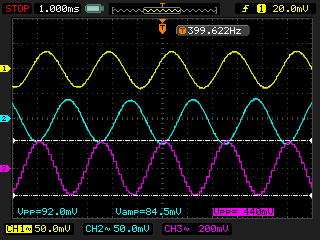
\includegraphics[scale=0.7]{../Assets/Results/1_400_3_off.png}
		\caption{Przebieg sygnałów przy wyłączonym algorytmie aktywnego tłumienia hałasu dla pomiaru~1.}
		\label{fig:test_1_off}
	\end{figure}
	\begin{figure}[h!]
		\centering
		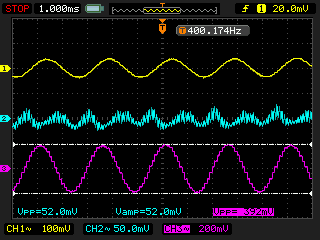
\includegraphics[scale=0.7]{../Assets/Results/1_400_3_on.png}
		\caption{Przebieg sygnałów przy włączonym algorytmie aktywnego tłumienia hałasu dla pomiaru~1.}
		\label{fig:test_1_on}
	\end{figure}
	W~pierwszym pomiarze sprawdzono charakter pracy urządzenia dla częstotliwości z~dolnych granic możliwości prototypu. Ponieważ zapewniono niski poziom natężenia hałasu, który nie wprawiał elementów konstrukcji w~nadmierne drgania własne, to filtr był w~stanie efektywnie wytłumić dźwięk wewnątrz komory. Można zauważyć pojawiające się przesterowania głośnika (charakteryzujące się nierównomiernym kształtem fali odbieranej przez mikrofon odsłuchowy na kanale drugim oscyloskopu), które wraz ze wzrostem natężenia dźwięku wejściowego narastają, rozstrajając filtr. Ostatecznie, porównując amplitudę sygnału na kanale drugim dla obu przypadków (z~tłumieniem aktywnym wyłączonym i~włączonym), można obliczyć według wzoru $20log(\frac{V_2}{V_1})$, o~ile stłumiono hałas. W~tym przypadku osiągnięto redukcję na poziomie około \SI{4,2}{\dB}.
	\item Test sinusoidy o~częstotliwości równej \SI{579}{\Hz}, wartości międzyszczytowej równej 5~$V_{pp}$ (rys. \ref{fig:test_2_off}, \ref{fig:test_2_on}).\\
	\begin{figure}[h!]
		\centering
		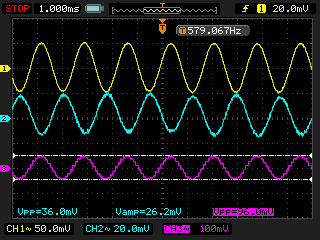
\includegraphics[scale=0.7]{../Assets/Results/2_579_5_off.png}
		\caption{Przebieg sygnałów przy wyłączonym algorytmie aktywnego tłumienia hałasu dla pomiaru~2.}
		\label{fig:test_2_off}
	\end{figure}
	\begin{figure}[h!]
		\centering
		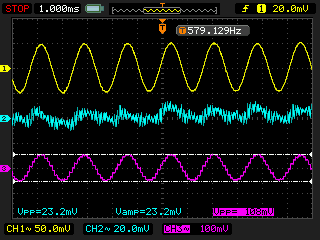
\includegraphics[scale=0.7]{../Assets/Results/2_579_5_on.png}
		\caption{Przebieg sygnałów przy włączonym algorytmie aktywnego tłumienia hałasu dla pomiaru~2.}
		\label{fig:test_2_on}
	\end{figure}
	Dla drugiego testu wybrano częstotliwość ze środkowej części pasma urządzenia i~nieco zwiększono amplitudę sygnału wejściowego. Również w~tym przypadku udało się wytłumić hałas, choć wciąż zauważalne są drobne przesterowania. Udało się obniżyć poziom natężenia niepożądanego dźwięku o~około \SI{1}{\dB}.
	\item Test sinusoidy o~częstotliwości równej \SI{820}{\Hz}, wartości międzyszczytowej równej 8~$V_{pp}$ (rys. \ref{fig:test_3_off}, \ref{fig:test_3_on}).\\
	\begin{figure}[h!]
		\centering
		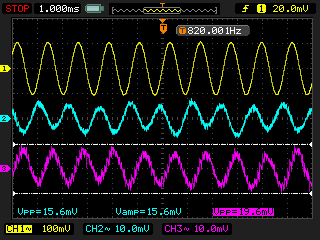
\includegraphics[scale=0.7]{../Assets/Results/3_820_8_off.png}
		\caption{Przebieg sygnałów przy wyłączonym algorytmie aktywnego tłumienia hałasu dla pomiaru~3.}
		\label{fig:test_3_off}
	\end{figure}
	\begin{figure}[h!]
		\centering
		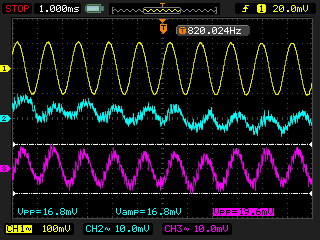
\includegraphics[scale=0.7]{../Assets/Results/3_820_8_on.png}
		\caption{Przebieg sygnałów przy włączonym algorytmie aktywnego tłumienia hałasu dla pomiaru~3.}
		\label{fig:test_3_on}
	\end{figure}
	W~tej części testowano górną granicę efektywnego tłumienia. Zniekształcenia od głośnika są nieco mniej zauważalne w~sygnale, widać jednak malejący wpływ metody aktywnej na hałas o~wyższych częstotliwościach. Obniżenie poziomu hałasu wyniosło tutaj \SI{+0,64}{\dB}, a~więc wydawałoby się, że sygnał został wzmocniony. Jednak wizualna analiza przebiegów na zrzutach ekranu oscyloskopu każe uznać skuteczność tłumienia. Niekorzystny wynik liczbowy jest zapewne skutkiem powolnego dryfowania sygnału z~mikrofonu odsłuchowego podczas drugiego pomiaru.
	\item Test sinusoidy o~częstotliwości równej \SI{250}{\Hz}, wartości międzyszczytowej równej 6~$V_{pp}$ (rys. \ref{fig:test_4_off}, \ref{fig:test_4_on}).\\
	\begin{figure}[h!]
		\centering
		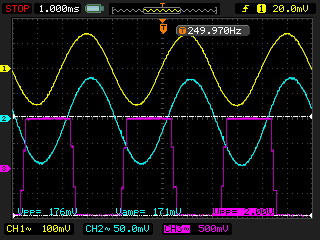
\includegraphics[scale=0.7]{../Assets/Results/4_250_6_off.png}
		\caption{Przebieg sygnałów przy wyłączonym algorytmie aktywnego tłumienia hałasu dla pomiaru~4.}
		\label{fig:test_4_off}
	\end{figure}
	\begin{figure}[h!]
		\centering
		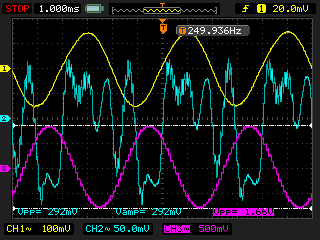
\includegraphics[scale=0.7]{../Assets/Results/4_250_6_on_notworking.png}
		\caption{Przebieg sygnałów przy włączonym algorytmie aktywnego tłumienia hałasu dla pomiaru~4.}
		\label{fig:test_4_on}
	\end{figure}
	Tutaj autor starał się ukazać zachowanie układu, który zostaje rozstrojony przez ,,zły'' typ hałasu. Dźwięk został w~tym przypadku wzmocniony o~\SI{4,65}{\dB}. Na wykresie widać wyraźnie wpływ zjawisk nieliniowych i~rezonansowych wnoszonych przez głośnik, które ujawniły się ze względu na jego przesterowanie. Widać wyraźnie wpływ nieliniowości głośnika, gdyż w~sygnale odsłuchowym pojawiły się składowe częstotliwości nieobecne ani w~hałasie zewnętrznym, ani w~sygnale podanym na głośnik wewnętrzny.
	\item Test sygnału prostokątnego o~częstotliwości \SI{720}{\Hz}, wartości międzyszczytowej równej 3~Vpp (rys. \ref{fig:test_5_off}, \ref{fig:test_5_on}).\\
	\begin{figure}[h!]
		\centering
		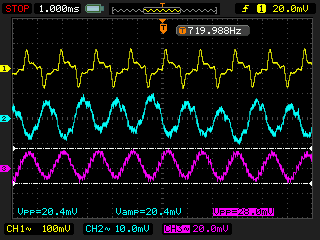
\includegraphics[scale=0.7]{../Assets/Results/5_720_3_sq_off.png}
		\caption{Przebieg sygnałów przy wyłączonym algorytmie aktywnego tłumienia hałasu dla pomiaru~5.}
		\label{fig:test_5_off}
	\end{figure}
	\begin{figure}[h!]
		\centering
		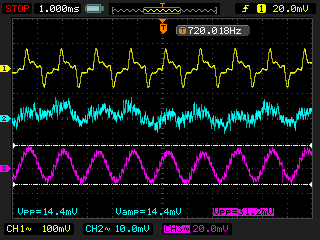
\includegraphics[scale=0.7]{../Assets/Results/5_720_3_sq_on.png}
		\caption{Przebieg sygnałów przy włączonym algorytmie aktywnego tłumienia hałasu dla pomiaru~5.}
		\label{fig:test_5_on}
	\end{figure}
	W~następnym etapie przetestowano falę prostokątną, której charakter brzmieniowy znacznie różni się od fali sinusoidalnej. Okazało się, że po pewnym czasie (dłuższym niż poprzednim razem) filtr jest w~stanie wytłumić również i~taki typ hałasu. Poziom obniżenia hałasu szacuje się na \SI{-3}{\dB}. Ponieważ przebieg tego sygnału jest ciekawszy od czystego harmonicznie sinusa, zapisano wagi filtra LMS i~na ich podstawie wygenerowano wykres odpowiedzi impulsowej filtra, który przedstawiony jest na rys. \ref{fig:test_5_lms}.
	\begin{figure}[h!]
		\centering
		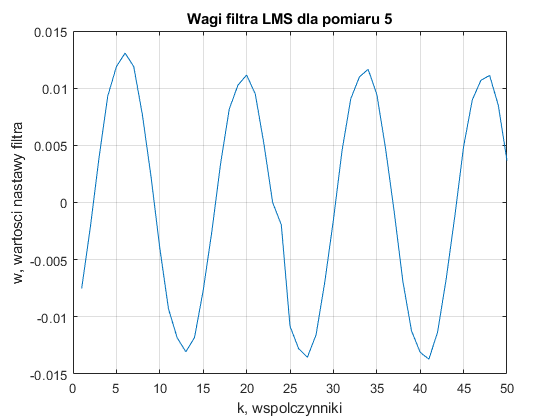
\includegraphics[scale=0.8]{../Assets/Results/5_wagi_lms.png}
		\caption{Odpowiedź impulsowa filtra dla pomiaru~5.}
		\label{fig:test_5_lms}
	\end{figure}
	\item Test sygnału będącego sumą sinusoidy 1~o~częstotliwości równej \SI{451}{\Hz}, wartości międzyszczytowej równej 3,1~$V_{pp}$ oraz sinusoidy 2~o~częstotliwości \SI{627}{\Hz}, wartości międzyszczytowej równej 6,6~$V_{pp}$ (rys. \ref{fig:test_6_off}, \ref{fig:test_6_on}).\\
	\begin{figure}[h!]
		\centering
		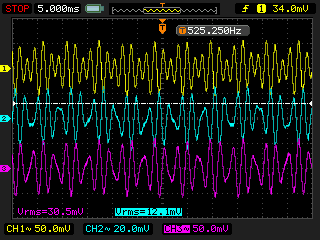
\includegraphics[scale=0.7]{../Assets/Results/6_complex_off.png}
		\caption{Przebieg sygnałów przy wyłączonym algorytmie aktywnego tłumienia hałasu dla pomiaru~6.}
		\label{fig:test_6_off}
	\end{figure}	
	\begin{figure}[h!]
		\centering
		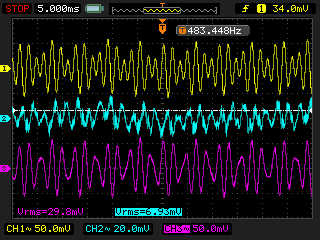
\includegraphics[scale=0.7]{../Assets/Results/6_complex_on.png}
		\caption{Przebieg sygnałów przy włączonym algorytmie aktywnego tłumienia hałasu dla pomiaru~6.}
		\label{fig:test_6_on}
	\end{figure}
	W~przypadku tego testu postanowiono sprawdzić zachowanie filtra przy obecności złożonego źródła hałasu -- co najmniej dwóch różnych sygnałów sinusoidalnych podanych jednocześnie na głośnik. Okazało się, że filtr pomimo bardzo długiego czasu uczenia (można by tutaj zwiększyć parametr $\beta$ algorytmu, ale istnieje ryzyko jego rozregulowania takimi operacjami) jest w~stanie dobrze stłumić taki dźwięk. Porównując parametry $V_{rms}$, filtr po uruchomieniu tłumienia obniża poziom takiego hałasu o~\SI{4,84}{\dB}. Również w~tym przypadku zdecydowano się na zapisanie wag filtra i~wygenerowanie na ich podstawie odpowiedzi impulsowej filtra, którą znaleźć można na rysunku \ref{fig:test_6_lms}.
	\begin{figure}[h!]
		\centering
		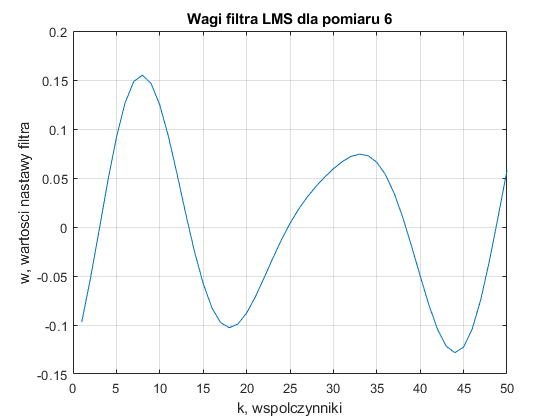
\includegraphics[scale=0.8]{../Assets/Results/6_wagi_lms.png}
		\caption{Odpowiedź impulsowa filtra dla pomiaru~6.}
		\label{fig:test_6_lms}
\end{figure}
	\item Test sygnału ,,sweep'' przy wyłączonym algorytmie.\\
	Ostatni z~testów miał na celu wyznaczenie charakterystyki Bodego pasywnej osłony dźwiękochłonnej użytej w~projekcie. ,,Przemiatano'' częstotliwości w~zakresie efektywnego tłumienia urządzenia, jednak przy wyłączonym algorytmie. W~tym teście głównym celem było ukazanie faktycznych różnic w~zastosowaniu pasywnego oraz aktywnego tłumienia. Wyznaczona w~ten sposób charakterystyka znajduje się na rysunku \ref{fig:bode}.
	\begin{figure}[h!]
		\centering
		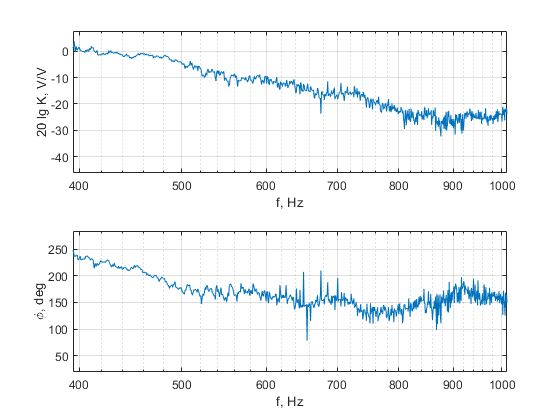
\includegraphics[scale=0.9]{../Assets/bode_przegrode.png}
		\caption{Charakterystyka Bodego przegrody dźwiękochłonnej.}
		\label{fig:bode}
	\end{figure}

Zgodnie z~omawianymi w~rozdziale \ref{cha:teoria} różnicami, na wspomnianej charakterystyce można zauważyć, że skuteczność tłumienia nauszników pasywnych wzrasta razem z~częstotliwością sygnału do wytłumienia. Aby wyznaczyć charakterystyki częstotliwościowe, porównano napięcie przesyłane przez mikrofon feedforward z~napięciem pochodzącym z~mikrofonu feedback. Wykres ten przedstawiony jest tutaj głównie jako ciekawy dodatek i~wyjaśnienie kwestii tłumienia pasywnego. Pozostaje on jednak do dalszego zgłębienia, bowiem pomimo faktu, iż autor nie potrzebował znać dokładnych parametrów przegrody w~tym projekcie, to znajomość tej charakterystyki może być przydatna w~dalszych iteracjach i~usprawnieniach urządzenia oraz w~badaniach symulacyjnych.
\end{enumerate}